% answers.tex —— 2020 年·北京卷 · 参考答案与详细解析片段
% 由 tools/generate_projects.py 依来源总账自 2020/2020_数学真题_北京_试题.md + 2020/2020_数学真题_北京_解析正文.md + 2020/2020_数学真题_北京_答案要点.md 生成，勿手改（改源 MD 后重跑）


\begin{answer}
\gksolhead{1}{}

\textbf{题目}：

已知集合 $A=\{-1,0,1,2\}$，$B=\{x\mid 0<x<3\}$，则 $A\cap B=$\mbox{（　　）}

（A）$\{-1,0,1\}$；（B）$\{0,1\}$；（C）$\{-1,1,2\}$；（D）$\{1,2\}$。

\Needspace{4\baselineskip}
\textbf{解析}

\Needspace{5\baselineskip}
$B=\{x\mid0<x<3\}$ 中的整数只有 $1$ 与 $2$，在 $A=\{-1,0,1,2\}$ 中筛出 $1$、$2$，故
\nopagebreak[4]
\[A\cap B=\{1,2\},\]
选 D。

\gkanswer{答案：D。$0<x<3$ 中的整数为 $1$、$2$，故 $A\cap B=\{1,2\}$。}

\end{answer}
\begin{answer}
\gksolhead{2}{}

\textbf{题目}：

在复平面内，复数 $z$ 对应的点的坐标是 $(1,2)$，则 $\mathrm i\cdot z=$\mbox{（　　）}

（A）$1+2\mathrm i$；（B）$-2+\mathrm i$；（C）$1-2\mathrm i$；（D）$-2-\mathrm i$。

\Needspace{4\baselineskip}
\textbf{解析}

\Needspace{5\baselineskip}
复数 $z$ 对应的点为 $(1,2)$，故 $z=1+2\mathrm i$。乘以 $\mathrm i$ 相当于把该点绕原点逆时针旋转 $90^\circ$，用代数式计算更直接：
\nopagebreak[4]
\[\mathrm i\cdot z=\mathrm i(1+2\mathrm i)=\mathrm i+2\mathrm i^2=-2+\mathrm i .\]
选 B。

\gkanswer{答案：B。$z=1+2\mathrm i$，$\mathrm i\cdot z=\mathrm i-2=-2+\mathrm i$。}

\end{answer}
\begin{answer}
\gksolhead{3}{}

\textbf{题目}：

在 $(\sqrt x-2)^5$ 的展开式中，$x^2$ 的系数为\mbox{（　　）}

（A）$-5$；（B）$5$；（C）$-10$；（D）$10$。

\Needspace{4\baselineskip}
\textbf{解析}

\Needspace{5\baselineskip}
展开式的通项为
\nopagebreak[4]
\[T_{k+1}=\mathrm C_5^k\left(\sqrt x\right)^{5-k}(-2)^k=\mathrm C_5^k(-2)^k x^{\frac{5-k}2},\qquad k=0,1,\cdots,5 .\]
\Needspace{5\baselineskip}
要求 $x^2$ 项，令 $\dfrac{5-k}2=2$，得 $k=1$。故 $x^2$ 的系数为
\nopagebreak[4]
\[\mathrm C_5^1\cdot(-2)=-10 .\]
选 C。若误令 $\dfrac{5-k}2$ 为其它值，会得到 $-5$、$5$、$10$ 等干扰项。

\gkanswer{答案：C。通项 $\mathrm C_5^k(\sqrt x)^{5-k}(-2)^k$，令 $\dfrac{5-k}2=2$ 得 $k=1$，系数 $\mathrm C_5^1\cdot(-2)=-10$。}

\end{answer}
\begin{answer}
\gksolhead{4}{}

\textbf{题目}：

某三棱柱的底面为正三角形，其三视图如图所示，该三棱柱的表面积为\mbox{（　　）}

（A）$6+\sqrt3$；（B）$6+2\sqrt3$；（C）$12+\sqrt3$；（D）$12+2\sqrt3$。
\nopagebreak[4]
\begin{center}% 2020 北京卷 第 4 题：正三棱柱的三视图
% 来源 PDF：普通高考/2020/2020北京.pdf 第 1 页（A3 横排），印面 1113，第 4 题题干下方
% 原页矢量（pt，左上角为原点）：正（主）视图为 62.37 x 62.36 的正方形，中线一条竖直虚线；
%   侧（左）视图为同尺寸正方形；俯视图为底边 62.37、高 62.36 的等腰三角形（顶点在上）；
%   尺寸标注：左侧竖直双箭头「2」，主视图底边在中线处分为「1」「1」两段。
% 说明：原页三视图为示意画法（侧视图宽度与主视图相同、俯视图高等于底边），并非严格按
%   正三角形的高 sqrt3 缩放；题干另以「底面为正三角形」和尺寸 2、1、1 给出真实数据，
%   即底面正三角形边长 2、棱柱高 2。此处按原页如实重绘，不据图量取比例。
\begin{tikzpicture}[line width=0.7pt, font=\small,
  x=1.05cm, y=1.05cm, line cap=round, line join=round]

  % 正（主）视图：2 x 2 正方形 + 中线竖直虚线
  \draw (0,0) rectangle (2,2);
  \draw[dashed] (1,0) -- (1,2);

  % 侧（左）视图：2 x 2 正方形
  \draw (3,0) rectangle (5,2);

  % 俯视图：底边 2、顶点在上的等腰三角形（原页画法）
  \draw (0,-3.05) -- (2,-3.05) -- (1,-1.05) -- cycle;

  % 尺寸标注：高 2（左侧竖直双箭头）
  \draw[<->] (-0.30,0) -- (-0.30,2);
  \draw[thin] (-0.40,0) -- (0,0);
  \draw[thin] (-0.40,2) -- (0,2);
  \node[left, inner sep=3pt] at (-0.32,1) {$2$};

  % 尺寸标注：底边 1 与 1
  \draw[<->] (0,-0.24) -- (1,-0.24);
  \draw[<->] (1,-0.24) -- (2,-0.24);
  \node[below=1pt, inner sep=0pt] at (0.5,-0.24) {$1$};
  \node[below=1pt, inner sep=0pt] at (1.5,-0.24) {$1$};

  % 视图名称
  \node[below=2pt, inner sep=0pt] at (1,-0.72) {正（主）视图};
  \node[below=2pt, inner sep=0pt] at (4,-0.72) {侧（左）视图};
  \node[below=2pt, inner sep=0pt] at (1,-3.22) {俯视图};
\end{tikzpicture}
\end{center}
\nopagebreak[4]
\Needspace{4\baselineskip}
\textbf{解析}

由三视图还原几何体。正（主）视图是边长 $2$ 的正方形，其中一条竖直虚线是棱柱后侧那条棱的投影，说明棱柱的高为 $2$，且侧面正对观察者的是宽度为 $2$ 的矩形；侧（左）视图同样是边长 $2$ 的正方形；俯视图为正三角形，底边上标注 $1$ 与 $1$，故底面正三角形的边长为 $1+1=2$。于是该几何体是底面边长 $2$、侧棱长（即高）$2$ 的正三棱柱。

\Needspace{5\baselineskip}
表面积由两个底面与三个侧面组成：
\nopagebreak[4]
\[S=2\times\frac{\sqrt3}4\times2^2+3\times(2\times2)=2\sqrt3+12 .\]
选 D。

\begin{gktip}
注：原页三视图为示意画法，侧视图宽度与主视图相同、俯视图的高也画成与底边相等，都不严格等于正三角形的高 $\sqrt3$；真实尺寸以题干「底面为正三角形」与标注 $2$、$1$、$1$ 为准，不能靠量图取比例。
\end{gktip}

\gkanswer{答案：D。由三视图知底面正三角形边长 $2$、侧棱长 $2$，表面积 $3\times(2\times2)+2\times\dfrac{\sqrt3}4\times2^2=12+2\sqrt3$。}

\end{answer}
\begin{answer}
\gksolhead{5}{}

\textbf{题目}：

已知半径为 $1$ 的圆经过点 $(3,4)$，则其圆心到原点的距离的最小值为\mbox{（　　）}

（A）$4$；（B）$5$；（C）$6$；（D）$7$。

\Needspace{4\baselineskip}
\textbf{解析}

\Needspace{5\baselineskip}
设圆心为 $C$。圆半径为 $1$ 且经过 $P(3,4)$，故 $|CP|=1$，即 $C$ 的轨迹是以 $P$ 为心、$1$ 为半径的圆。设 $O$ 为原点，$|OP|=\sqrt{3^2+4^2}=5$，由三角不等式
\nopagebreak[4]
\[|OC|\geqslant|OP|-|CP|=5-1=4,\]
当 $C$ 落在线段 $OP$ 上（即 $C$ 为 $OP$ 与轨迹圆的交点）时取等号。故最小值为 $4$，选 A。

\gkanswer{答案：A。圆心轨迹是以 $(3,4)$ 为心、$1$ 为半径的圆，圆心到原点距离最小为 $5-1=4$。}

\end{answer}
\begin{answer}
\gksolhead{6}{}

\textbf{题目}：

已知函数 $f(x)=2^x-x-1$，则不等式 $f(x)>0$ 的解集是\mbox{（　　）}

（A）$(-1,1)$；（B）$(-\infty,-1)\cup(1,+\infty)$；（C）$(0,1)$；（D）$(-\infty,0)\cup(1,+\infty)$。

\Needspace{4\baselineskip}
\textbf{解析}

\Needspace{5\baselineskip}
不等式 $f(x)>0$ 即 $2^x>x+1$。令 $g(x)=2^x-x-1$，则 $g(0)=0$，$g(1)=0$，且
\nopagebreak[4]
\[g'(x)=2^x\ln2-1,\qquad g''(x)=2^x(\ln2)^2>0,\]
\Needspace{5\baselineskip}
故 $g'$ 严格递增，存在唯一零点 $x_0=\log_2\dfrac1{\ln2}\approx0.53$，$g$ 在 $(-\infty,x_0)$ 递减、在 $(x_0,+\infty)$ 递增。于是 $g$ 恰有两个零点 $0$ 与 $1$，且
\nopagebreak[4]
\[g(x)>0\iff x<0\ \text{\text{或}}\ x>1 .\]
解集为 $(-\infty,0)\cup(1,+\infty)$，选 D。

\gkanswer{答案：D。$2^x>x+1$ 在两图象交点 $(0,1)$、$(1,2)$ 之外成立，解集为 $(-\infty,0)\cup(1,+\infty)$。}

\end{answer}
\begin{answer}
\gksolhead{7}{}

\textbf{题目}：

设抛物线的顶点为 $O$，焦点为 $F$，准线为 $l$。$P$ 是抛物线上异于 $O$ 的一点，过 $P$ 作 $PQ\perp l$ 于 $Q$，则线段 $FQ$ 的垂直平分线\mbox{（　　）}

（A）经过点 $O$；（B）经过点 $P$；（C）平行于直线 $OP$；（D）垂直于直线 $OP$。

\Needspace{4\baselineskip}
\textbf{解析}

\Needspace{5\baselineskip}
设抛物线焦点为 $F$、准线为 $l$。由抛物线的定义，抛物线上任一点到焦点的距离等于它到准线的距离，故对题中的 $P$ 有
\nopagebreak[4]
\[|PF|=d(P,l)=|PQ| .\]
于是 $P$ 到 $F$、$Q$ 两点距离相等，$P$ 落在线段 $FQ$ 的垂直平分线上，即该垂直平分线经过点 $P$。

其余选项不成立：以 $y^2=4x$ 为例，$F(1,0)$，取 $P(1,2)$，则 $Q(-1,2)$，$FQ$ 的中点为 $(0,1)$，垂直平分线为 $y=x+1$，它不过原点 $O(0,0)$（排除 A）；其斜率为 $1$，而 $OP$ 斜率为 $2$，既不平行也不垂直（排除 C、D）。选 B。

\gkanswer{答案：B。由抛物线定义 $|PF|=|PQ|$，故 $P$ 在 $FQ$ 的垂直平分线上。}

\end{answer}
\begin{answer}
\gksolhead{8}{}

\textbf{题目}：

在等差数列 $\{a_n\}$ 中，$a_1=-9$，$a_3=-1$。记 $T_n=a_1a_2\cdots a_n$（$n=1,2,\cdots$），则数列 $\{T_n\}$\mbox{（　　）}

（A）有最大项，有最小项；（B）有最大项，无最小项；

（C）无最大项，有最小项；（D）无最大项，无最小项。

\Needspace{4\baselineskip}
\textbf{解析}

\Needspace{5\baselineskip}
设公差为 $d$，由 $a_1=-9$、$a_3=-1$ 得 $2d=a_3-a_1=8$，故 $d=4$，
\nopagebreak[4]
\[a_n=-9+4(n-1)=4n-13 .\]
\Needspace{5\baselineskip}
于是 $a_1=-9$，$a_2=-5$，$a_3=-1$，$a_4=3$，$a_5=7,\cdots$，前 $3$ 项为负、从第 $4$ 项起为正。逐项算出
\nopagebreak[4]
\[T_1=-9,\quad T_2=45,\quad T_3=-45,\quad T_4=-135 .\]
\Needspace{5\baselineskip}
当 $n\geqslant5$ 时 $a_n\geqslant7>1$，故
\nopagebreak[4]
\[T_n=T_4\cdot a_5a_6\cdots a_n ,\]
其绝对值随 $n$ 严格增大而符号恒为负，因此 $T_n$ 自 $n=4$ 起单调递减、无下界，即\textbf{无最小项}；而 $T_2=45$ 大于全部 $T_n$（$n\neq2$ 时或为负、或为 $-9$），故\textbf{有最大项} $45$。

选 B。（若误把条件读成 $a_5=-1$，则 $d=2$、$a_n=2n-11$，符号结构相同，结论仍是「有最大项、无最小项」。）

\gkanswer{答案：B。公差 $d=\dfrac{a_3-a_1}2=4$，$a_n=4n-13$；$T_1=-9$，$T_2=45$ 为最大项，$T_4=-135$ 起全为负且绝对值递增，故无最小项。}

\end{answer}
\begin{answer}
\gksolhead{9}{}

\textbf{题目}：

已知 $\alpha$，$\beta\in\mathbf R$，则「存在 $k\in\mathbf Z$ 使得 $\alpha=k\pi+(-1)^k\beta$」是「$\sin\alpha=\sin\beta$」的\mbox{（　　）}

（A）充分而不必要条件；（B）必要而不充分条件；（C）充分必要条件；（D）既不充分也不必要条件。

\Needspace{4\baselineskip}
\textbf{解析}

先证充分性。若存在 $k\in\mathbf Z$ 使 $\alpha=k\pi+(-1)^k\beta$：

\begin{itemize}
\item $k=2n$ 为偶数时 $\alpha=2n\pi+\beta$，故 $\sin\alpha=\sin(2n\pi+\beta)=\sin\beta$；
\item $k=2n+1$ 为奇数时 $\alpha=2n\pi+\pi-\beta$，故 $\sin\alpha=\sin(\pi-\beta)=\sin\beta$。
\end{itemize}

\Needspace{5\baselineskip}
再证必要性。若 $\sin\alpha=\sin\beta$，则 $\alpha$ 与 $\beta$ 的终边相同或关于 $y$ 轴对称，即
\nopagebreak[4]
\[\alpha=2n\pi+\beta\quad\text{\text{或}}\quad\alpha=2n\pi+\pi-\beta\qquad(n\in\mathbf Z),\]
前者取 $k=2n$，后者取 $k=2n+1$，统一写作 $\alpha=k\pi+(-1)^k\beta$。

两方向都成立，故为充分必要条件，选 C。

\gkanswer{答案：C。$k$ 为偶数时 $\alpha=2n\pi+\beta$、为奇数时 $\alpha=2n\pi+\pi-\beta$，两式恰覆盖 $\sin\alpha=\sin\beta$ 的全部情形，故为充要条件。}

\end{answer}
\begin{answer}
\gksolhead{10}{}

\textbf{题目}：

2020 年 3 月 14 日是全球首个国际圆周率日（$\pi$ Day）。历史上，求圆周率 $\pi$ 的方法有多种，与中国传统数学中的「割圆术」相似。数学家阿尔·卡西的方法是：当正整数 $n$ 充分大时，计算单位圆的内接正 $6n$ 边形的周长和外切正 $6n$ 边形（各边均与圆相切的正 $6n$ 边形）的周长，将它们的算术平均数作为 $2\pi$ 的近似值。按照阿尔·卡西的方法，$\pi$ 的近似值的表达式是\mbox{（　　）}

（A）$3n\left(\sin\dfrac{30^\circ}{n}+\tan\dfrac{30^\circ}{n}\right)$；（B）$6n\left(\sin\dfrac{30^\circ}{n}+\tan\dfrac{30^\circ}{n}\right)$；

（C）$3n\left(\sin\dfrac{60^\circ}{n}+\tan\dfrac{60^\circ}{n}\right)$；（D）$6n\left(\sin\dfrac{60^\circ}{n}+\tan\dfrac{60^\circ}{n}\right)$。

\Needspace{4\baselineskip}
\textbf{解析}

\Needspace{5\baselineskip}
单位圆的内接正 $6n$ 边形，每条边所对圆心角为 $\dfrac{2\pi}{6n}=\dfrac{60^\circ}{n}$，故边长
\nopagebreak[4]
\[a=2\sin\frac{30^\circ}{n},\qquad \text{\text{周长}}=6n\cdot a=12n\sin\frac{30^\circ}{n}.\]
\Needspace{5\baselineskip}
外切正 $6n$ 边形的边与圆相切，边心距为 $1$，故边长
\nopagebreak[4]
\[b=2\tan\frac{30^\circ}{n},\qquad \text{\text{周长}}=12n\tan\frac{30^\circ}{n}.\]
\Needspace{5\baselineskip}
按题意取两者算术平均数作为 $2\pi$ 的近似值：
\nopagebreak[4]
\[2\pi\approx\frac{12n\sin\frac{30^\circ}{n}+12n\tan\frac{30^\circ}{n}}2=6n\left(\sin\frac{30^\circ}{n}+\tan\frac{30^\circ}{n}\right),\]
\Needspace{5\baselineskip}
两边除以 $2$ 得
\nopagebreak[4]
\[\pi\approx3n\left(\sin\frac{30^\circ}{n}+\tan\frac{30^\circ}{n}\right).\]
选 A。B 项漏除了 $2$，C、D 项把圆心角的一半误取为 $\dfrac{60^\circ}{n}$。

数值复核：取 $n=1000$，$3n\left(\sin0.03^\circ+\tan0.03^\circ\right)=3000(5.23599\times10^{-4}+5.23599\times10^{-4})\approx3.14159$，与 $\pi$ 相符。

\gkanswer{答案：A。内接正 $6n$ 边形周长 $12n\sin\dfrac{30^\circ}n$，外切周长 $12n\tan\dfrac{30^\circ}n$，二者平均为 $2\pi$ 的近似值，故 $\pi\approx3n\left(\sin\dfrac{30^\circ}n+\tan\dfrac{30^\circ}n\right)$。}

\end{answer}
\begin{answer}
\gksolhead{11}{}

\textbf{题目}：

函数 $f(x)=\dfrac1{x+1}+\ln x$ 的定义域是\gkblank{}。

\Needspace{4\baselineskip}
\textbf{解析}

\Needspace{5\baselineskip}
解析式含 $\dfrac1{x+1}$ 与 $\ln x$ 两部分，须同时有意义：
\nopagebreak[4]
\[x+1\neq0\quad\text{\text{且}}\quad x>0 .\]
$x>0$ 已蕴含 $x\neq-1$，故定义域为 $(0,+\infty)$。

\gkanswer{答案：$(0,+\infty)$。需 $x+1\neq0$ 且 $x>0$，故定义域为 $(0,+\infty)$。}

\end{answer}
\begin{answer}
\gksolhead{12}{}

\textbf{题目}：

已知双曲线 $C:\dfrac{x^2}6-\dfrac{y^2}3=1$，则 $C$ 的右焦点的坐标为\gkblank{}；$C$ 的焦点到其渐近线的距离是\gkblank{}。

\Needspace{4\baselineskip}
\textbf{解析}

\Needspace{5\baselineskip}
双曲线 $\dfrac{x^2}6-\dfrac{y^2}3=1$ 中 $a^2=6$，$b^2=3$，故
\nopagebreak[4]
\[c=\sqrt{a^2+b^2}=\sqrt{6+3}=3,\]
右焦点为 $(3,0)$。

\Needspace{5\baselineskip}
渐近线由 $\dfrac{x^2}6-\dfrac{y^2}3=0$ 得 $y=\pm\dfrac{x}{\sqrt2}$，即 $x\mp\sqrt2\,y=0$。焦点 $(3,0)$ 到渐近线的距离为
\nopagebreak[4]
\[d=\frac{|3|}{\sqrt{1+2}}=\frac3{\sqrt3}=\sqrt3 .\]
两空依次填 $(3,0)$、$\sqrt3$。

\gkanswer{答案：$(3,0)$；$\sqrt3$。$c^2=6+3=9$，右焦点 $(3,0)$；渐近线 $y=\dfrac{x}{\sqrt2}$，距离 $\dfrac3{\sqrt3}=\sqrt3$。}

\end{answer}
\begin{answer}
\gksolhead{13}{}

\textbf{题目}：

已知正方形 $ABCD$ 的边长为 $2$，点 $P$ 满足 $\overrightarrow{AP}=\dfrac12\left(\overrightarrow{AB}+\overrightarrow{AC}\right)$，则 $|\overrightarrow{PD}|=$\gkblank{}；$\overrightarrow{PB}\cdot\overrightarrow{PD}=$\gkblank{}。

\Needspace{4\baselineskip}
\textbf{解析}

\Needspace{5\baselineskip}
以 $A$ 为原点、$\overrightarrow{AB}$、$\overrightarrow{AD}$ 为 $x$、$y$ 轴正方向建系。边长为 $2$，则
\nopagebreak[4]
\[A(0,0),\quad B(2,0),\quad C(2,2),\quad D(0,2).\]
\Needspace{5\baselineskip}
由 $\overrightarrow{AP}=\dfrac12\left(\overrightarrow{AB}+\overrightarrow{AC}\right)$ 得
\nopagebreak[4]
\[\overrightarrow{AP}=\frac12\bigl((2,0)+(2,2)\bigr)=(2,1),\]
\Needspace{5\baselineskip}
故 $P(2,1)$。于是
\nopagebreak[4]
\[\overrightarrow{PD}=D-P=(-2,1),\qquad |\overrightarrow{PD}|=\sqrt{(-2)^2+1^2}=\sqrt5 ;\]
\nopagebreak[4]
\[\overrightarrow{PB}=B-P=(0,-1),\qquad \overrightarrow{PB}\cdot\overrightarrow{PD}=0\times(-2)+(-1)\times1=-1 .\]
两空依次填 $\sqrt5$、$-1$。

\gkanswer{答案：$\sqrt5$；$-1$。取 $A(0,0)$、$B(2,0)$、$C(2,2)$、$D(0,2)$，得 $P(2,1)$，故 $|\overrightarrow{PD}|=\sqrt{4+1}=\sqrt5$，$\overrightarrow{PB}\cdot\overrightarrow{PD}=(0,-1)\cdot(-2,1)=-1$。}

\end{answer}
\begin{answer}
\gksolhead{14}{}

\textbf{题目}：

若函数 $f(x)=\sin(x+\varphi)+\cos x$ 的最大值为 $2$，则常数 $\varphi$ 的一个取值为\gkblank{}。

\Needspace{4\baselineskip}
\textbf{解析}

\Needspace{5\baselineskip}
展开并合并同类项：
\nopagebreak[4]
\[\begin{aligned}
f(x)&=\sin(x+\varphi)+\cos x\\
&=\sin x\cos\varphi+\cos x\sin\varphi+\cos x\\
&=\cos\varphi\cdot\sin x+(1+\sin\varphi)\cos x .
\end{aligned}\]
\Needspace{5\baselineskip}
形如 $A\sin x+B\cos x$ 的函数最大值为 $\sqrt{A^2+B^2}$，故
\nopagebreak[4]
\[\sqrt{\cos^2\varphi+(1+\sin\varphi)^2}=2 .\]
\Needspace{5\baselineskip}
两边平方：
\nopagebreak[4]
\[\cos^2\varphi+1+2\sin\varphi+\sin^2\varphi=4\Longrightarrow 2+2\sin\varphi=4\Longrightarrow\sin\varphi=1 .\]
故 $\varphi=2k\pi+\dfrac\pi2$（$k\in\mathbf Z$），取一个值即 $\dfrac\pi2$。

\gkanswer{答案：$\dfrac\pi2$（答案不唯一，$\varphi=2k\pi+\dfrac\pi2$ 均可）。振幅平方为 $\cos^2\varphi+(1+\sin\varphi)^2=2+2\sin\varphi=4$，故 $\sin\varphi=1$。}

\end{answer}
\begin{answer}
\gksolhead{15}{}

\textbf{题目}：

为满足人民对美好生活的向往，环保部门要求相关企业加强污水治理，排放未达标的企业要限期整改。设企业的污水排放量 $W$ 与时间 $t$ 的关系为 $W=f(t)$，用 $-\dfrac{f(b)-f(a)}{b-a}$ 的大小评价在 $[a,b]$ 这段时间内企业污水治理能力的强弱。已知整改期内，甲、乙两企业的污水排放量与时间的关系如图所示。
\nopagebreak[4]
\begin{center}% 2020 北京卷 第 15 题：甲、乙两企业污水排放量 W 与时间 t 的关系曲线
% 来源 PDF：普通高考/2020/2020北京.pdf 第 1 页（A3 横排），印面 1113，第 15 题题干下方
% 重绘依据：原页该图为矢量路径，已由 pdftocairo -svg 解出四条折线（两企业各被 t2 处的
%   交点切成左右两段），按坐标轴端点（O、t 轴右端、W 轴上端）线性换算为本图坐标，
%   采样后以 plot 还原，形状与原页一致。
% 原页要素：横轴 t、纵轴 W；水平虚线「污水达标排放量」；t 轴上 t1、t2、t3 三条竖直虚线
%   （t1 在甲曲线开始明显下降之后、t2 在两曲线交点、t3 在两曲线都降到达标线以下之后）；
%   曲线起点处标「甲企业」（上）、「乙企业」（下），交点右下方标「乙企业」（上）、
%   「甲企业」（下）。
\begin{tikzpicture}[line width=0.7pt, font=\small,
  x=0.50cm, y=0.50cm, line cap=round, line join=round]

  % 坐标轴（W 轴比原页留高一点，供曲线标注）
  \draw[->] (0,0) -- (15.9,0) node[below, inner sep=5pt] {$t$};
  \draw[->] (0,0) -- (0,13.4) node[right, inner sep=3pt] {$W$};
  \node[below left, inner sep=2pt] at (0,0) {$O$};

  % 污水达标排放量（水平虚线；标注按原页置于纵轴左侧）
  \draw[dashed] (0,2.92) -- (15.1,2.92);
  \node[left, inner sep=2pt] at (-0.15,2.92) {污水达标排放量};

  % 甲企业曲线（左段：起点最高，先略升后下降；右段：过交点后降得最快）
  \draw plot[smooth] coordinates {
    (0.00,8.76) (0.82,8.86) (1.63,8.87) (2.45,8.79) (3.26,8.62)
    (4.07,8.37) (4.85,8.02) (5.62,7.60) (6.37,7.08) (7.10,6.49)
    (7.79,5.82) (8.45,5.08) (9.07,4.26)
  };
  \draw plot[smooth] coordinates {
    (9.07,4.26) (9.45,3.85) (9.83,3.47) (10.23,3.12) (10.64,2.80)
    (11.06,2.51) (11.49,2.26) (11.92,2.04) (12.37,1.85) (12.81,1.70)
    (13.27,1.58) (13.72,1.50) (14.18,1.46)
  };

  % 乙企业曲线（左段：起点较低，单调缓降；右段：过交点后仍在甲之上）
  \draw plot[smooth] coordinates {
    (0.00,6.60) (0.77,6.59) (1.54,6.55) (2.31,6.47) (3.08,6.36)
    (3.84,6.22) (4.60,6.04) (5.36,5.83) (6.11,5.58) (6.86,5.30)
    (7.61,4.99) (8.34,4.64) (9.07,4.26)
  };
  \draw plot[smooth] coordinates {
    (9.07,4.26) (9.47,3.98) (9.88,3.71) (10.29,3.47) (10.71,3.24)
    (11.13,3.05) (11.56,2.87) (11.99,2.72) (12.43,2.60) (12.86,2.50)
    (13.30,2.42) (13.74,2.37) (14.18,2.34)
  };

  % t1、t2、t3 三条竖直虚线（高度分别止于对应曲线）
  \draw[dashed] (3.89,0) -- (3.89,8.58);
  \draw[dashed] (9.07,0) -- (9.07,4.26);
  \draw[dashed] (13.80,0) -- (13.80,2.39);
  \node[below, inner sep=4pt] at (3.89,0) {$t_1$};
  \node[below, inner sep=4pt] at (9.07,0) {$t_2$};
  \node[below, inner sep=4pt] at (13.80,0) {$t_3$};

  % 曲线标注（按原页位置：起点标注在曲线上方，交点后的标注在右侧）
  \node[right, inner sep=2pt] at (0.45,10.18) {甲企业};
  \node[right, inner sep=2pt] at (0.45,7.85) {乙企业};
  \node[right, inner sep=2pt] at (10.95,4.62) {乙企业};
  \node[right, inner sep=2pt] at (10.95,1.52) {甲企业};
\end{tikzpicture}
\end{center}
\nopagebreak[4]
给出下列四个结论：

① 在 $[t_1,t_2]$ 这段时间内，甲企业的污水治理能力比乙企业强；

② 在 $t_2$ 时刻，甲企业的污水治理能力比乙企业强；

③ 在 $t_3$ 时刻，甲、乙两企业的污水排放都已达标；

④ 甲企业在 $[0,t_1]$、$[t_1,t_2]$、$[t_2,t_3]$ 这三段时间中，在 $[0,t_1]$ 的污水治理能力最强。

其中所有正确结论的序号是\gkblank{}。

\Needspace{4\baselineskip}
\textbf{解析}

题中「污水治理能力」用 $-\dfrac{f(b)-f(a)}{b-a}$ 度量，即该时段内排放量的\textbf{平均下降速率}，数值越大治理能力越强；在某一时刻则用瞬时下降速率（$|f'(t)|$，曲线越陡下降越快则能力越强）比较。

① 在 $[t_1,t_2]$ 内两条曲线都在下降，甲曲线从较高的位置降到交点，落差明显大于乙曲线在同一时段的落差，故甲的平均下降速率更大，甲企业治理能力更强。①正确。

② $t_2$ 时刻两曲线相交。交点的左侧甲在乙上方、右侧甲在乙下方，说明甲曲线在此处比乙曲线更陡地向下穿过交点，甲的瞬时下降速率更大。②正确。

③ $t_3$ 时刻，两曲线都位于「污水达标排放量」这条水平虚线之下，即两企业的排放量都已不超过达标排放量。③正确。

④ 甲的三个时段中，$[0,t_1]$ 段曲线几乎平坦（排放量基本没有下降），$[t_1,t_2]$ 段最陡，$[t_2,t_3]$ 段次之，故 $[0,t_1]$ 段的治理能力\textbf{最弱}而不是最强。④错误。

综上，正确结论的序号是 ①②③。

\gkanswer{答案：①②③。①区间平均下降速率甲大于乙；②$t_2$ 处甲曲线更陡且正由上方穿到下方；③$t_3$ 处两曲线均在达标线下方；④$[0,t_1]$ 段甲下降最缓，治理能力最弱，故④错。}

\end{answer}
\begin{answer}
\gksolhead{16}{}

\textbf{题目}：

如图，在正方体 $ABCD-A_1B_1C_1D_1$ 中，$E$ 为 $BB_1$ 的中点。

（1） 求证：$BC_1\parallel$ 平面 $AD_1E$；

（2） 求直线 $AA_1$ 与平面 $AD_1E$ 所成角的正弦值。
\nopagebreak[4]
\begin{center}% 2020 北京卷 第 16 题：正方体 ABCD-A1B1C1D1，E 为 BB1 的中点
% 来源 PDF：普通高考/2020/2020北京.pdf 第 1 页（A3 横排），印面 1113，第 16 题右侧
% 重绘依据：原页该图为矢量路径，pdftocairo -svg 解出全部端点后按棱长归一化逐个还原。
%   原页画法：前侧面为正方形 D1C1CD（D 在左下、C 在右下、C1 在右上、D1 在左上），
%   深度方向朝右上（斜二测，长度约为棱长的一半）；后侧面 A1B1BA 与前侧面平行，
%   A 是被遮挡的顶点，故 AA1、AB、AD、AD1、AE 画虚线，D1E 亦为虚线；
%   E 位于 BB1 的中点。
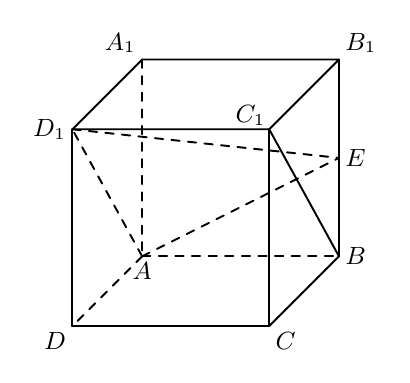
\begin{tikzpicture}[line width=0.7pt, font=\small,
  x=1.25cm, y=1.25cm, line cap=round, line join=round]

  % 顶点坐标（棱长 2，深度偏移 (0.709, 0.709)）
  \coordinate (D)  at (0.000, 0.000);
  \coordinate (C)  at (2.000, 0.000);
  \coordinate (C1) at (2.000, 2.000);
  \coordinate (D1) at (0.000, 2.000);
  \coordinate (A)  at (0.709, 0.709);
  \coordinate (B)  at (2.709, 0.709);
  \coordinate (B1) at (2.709, 2.709);
  \coordinate (A1) at (0.709, 2.709);
  \coordinate (E)  at (2.709, 1.709);

  % 上底面四边（实线）
  \draw (A1) -- (B1) -- (C1) -- (D1) -- cycle;

  % 可见棱（实线）
  \draw (D1) -- (D);
  \draw (C1) -- (C);
  \draw (D) -- (C);
  \draw (B1) -- (B);
  \draw (B) -- (C);
  \draw (B) -- (C1);

  % 被遮挡的棱与体内连线（虚线）
  \draw[dashed] (A1) -- (A);
  \draw[dashed] (A) -- (B);
  \draw[dashed] (A) -- (D);
  \draw[dashed] (A) -- (D1);
  \draw[dashed] (A) -- (E);
  \draw[dashed] (D1) -- (E);

  % 顶点标注
  \node[above left, inner sep=2pt]  at (A1) {$A_1$};
  \node[above right, inner sep=2pt] at (B1) {$B_1$};
  \node[above left, inner sep=1pt]  at (C1) {$C_1$};
  \node[left, inner sep=2pt]        at (D1) {$D_1$};
  \node[below, inner sep=2pt]       at (A)  {$A$};
  \node[right, inner sep=2pt]       at (B)  {$B$};
  \node[below right, inner sep=2pt] at (C)  {$C$};
  \node[below left, inner sep=2pt]  at (D)  {$D$};
  \node[right, inner sep=2pt]       at (E)  {$E$};
\end{tikzpicture}
\end{center}
\nopagebreak[4]
\Needspace{4\baselineskip}
\textbf{解析}

\gksubpart{（1）}

\Needspace{5\baselineskip}
在正方体中，$AD\parallel BC$ 且 $AD=BC$，$DD_1\parallel CC_1$ 且 $DD_1=CC_1$，于是
\nopagebreak[4]
\[\overrightarrow{AD_1}=\overrightarrow{AD}+\overrightarrow{DD_1}=\overrightarrow{BC}+\overrightarrow{CC_1}=\overrightarrow{BC_1},\]
\Needspace{5\baselineskip}
故 $AD_1\parallel BC_1$。又 $AD_1\subset$ 平面 $AD_1E$，而 $BC_1\not\subset$ 平面 $AD_1E$（点 $B$ 不在该平面内），由线面平行的判定定理得
\nopagebreak[4]
\[BC_1\parallel\text{\text{平面} }AD_1E .\]

\gksubpart{（2）}

\Needspace{5\baselineskip}
设棱长为 $2$，以 $A$ 为原点，$\overrightarrow{AB}$、$\overrightarrow{AD}$、$\overrightarrow{AA_1}$ 为 $x$、$y$、$z$ 轴正方向建系，则
\nopagebreak[4]
\[A(0,0,0),\quad B(2,0,0),\quad D_1(0,2,2),\quad A_1(0,0,2).\]
\Needspace{5\baselineskip}
$E$ 为 $BB_1$ 的中点，而 $B_1(2,0,2)$，故 $E(2,0,1)$。于是
\nopagebreak[4]
\[\overrightarrow{AD_1}=(0,2,2),\qquad \overrightarrow{AE}=(2,0,1).\]
\Needspace{5\baselineskip}
设平面 $AD_1E$ 的法向量为 $\boldsymbol n=(x,y,z)$，则
\nopagebreak[4]
\[\begin{cases}2y+2z=0,\\2x+z=0,\end{cases}\]
取 $z=-2$，得 $y=2$，$x=1$，即 $\boldsymbol n=(1,2,-2)$。

\Needspace{5\baselineskip}
又 $\overrightarrow{AA_1}=(0,0,2)$，设直线 $AA_1$ 与平面 $AD_1E$ 所成角为 $\theta$，则
\nopagebreak[4]
\[\sin\theta=\frac{\left|\overrightarrow{AA_1}\cdot\boldsymbol n\right|}{\left|\overrightarrow{AA_1}\right|\left|\boldsymbol n\right|}=\frac{|0+0-4|}{2\times\sqrt{1+4+4}}=\frac4{2\times3}=\frac23 .\]
所求正弦值为 $\dfrac23$。

\gkanswer{答案（1）：证明见解析。$\overrightarrow{BC_1}=\overrightarrow{AD_1}$，故 $BC_1\parallel AD_1\subset$ 平面 $AD_1E$，且 $BC_1$ 不在该平面内。}

\gkanswer{答案（2）：$\dfrac23$。平面 $AD_1E$ 的法向量取 $(1,2,-2)$，$\sin\theta=\dfrac{|\overrightarrow{AA_1}\cdot\boldsymbol n|}{|\overrightarrow{AA_1}||\boldsymbol n|}=\dfrac46=\dfrac23$。}

\end{answer}
\begin{answer}
\gksolhead{17}{}

\textbf{题目}：

在 $\triangle ABC$ 中，$a+b=11$，再从条件①、条件②这两个条件中选择一个作为已知，求：

（1） $a$ 的值；

（2） $\sin C$ 和 $\triangle ABC$ 的面积。

条件①：$c=7$，$\cos A=-\dfrac17$；

条件②：$\cos A=\dfrac18$，$\cos B=\dfrac9{16}$。

注：如果选择条件①和条件②分别解答，按第一个解答计分。

\Needspace{4\baselineskip}
\textbf{解析}

\gksubpart{（1）}

\Needspace{5\baselineskip}
\textbf{条件①}：$c=7$，$\cos A=-\dfrac17$，$a+b=11$。由余弦定理
\nopagebreak[4]
\[a^2=b^2+c^2-2bc\cos A=b^2+49-2\cdot b\cdot7\cdot\left(-\frac17\right)=b^2+2b+49 .\]
\Needspace{5\baselineskip}
代入 $a=11-b$：
\nopagebreak[4]
\[(11-b)^2=b^2+2b+49\Longrightarrow121-22b+b^2=b^2+2b+49\Longrightarrow72=24b,\]
故 $b=3$，$a=8$。

\Needspace{5\baselineskip}
\textbf{条件②}：$\cos A=\dfrac18$，$\cos B=\dfrac9{16}$，故
\nopagebreak[4]
\[\sin A=\sqrt{1-\frac1{64}}=\frac{3\sqrt7}8,\qquad \sin B=\sqrt{1-\frac{81}{256}}=\frac{5\sqrt7}{16}.\]
\Needspace{5\baselineskip}
由正弦定理 $a:b=\sin A:\sin B=\dfrac{3\sqrt7}8:\dfrac{5\sqrt7}{16}=6:5$，结合 $a+b=11$ 得
\nopagebreak[4]
\[a=6,\quad b=5 .\]

\gksubpart{（2）}

\Needspace{5\baselineskip}
\textbf{条件①}：由（1）$a=8$，$b=3$，$c=7$，且 $\sin A=\sqrt{1-\cos^2A}=\dfrac{4\sqrt3}7$。由正弦定理
\nopagebreak[4]
\[\sin C=\frac{c\sin A}{a}=\frac{7\times\frac{4\sqrt3}7}{8}=\frac{\sqrt3}2 .\]
\Needspace{5\baselineskip}
面积
\nopagebreak[4]
\[S=\frac12ab\sin C=\frac12\times8\times3\times\frac{\sqrt3}2=6\sqrt3 .\]

\Needspace{5\baselineskip}
\textbf{条件②}：由（1）$a=6$，$b=5$。因为 $C=\pi-(A+B)$，故
\nopagebreak[4]
\[\begin{aligned}
\cos C&=-\cos(A+B)=-\left(\cos A\cos B-\sin A\sin B\right)\\
&=-\left(\frac18\times\frac9{16}-\frac{3\sqrt7}8\times\frac{5\sqrt7}{16}\right)
=-\left(\frac9{128}-\frac{105}{128}\right)=\frac34,
\end{aligned}\]
\Needspace{5\baselineskip}
于是 $\sin C=\sqrt{1-\dfrac9{16}}=\dfrac{\sqrt7}4$。面积
\nopagebreak[4]
\[S=\frac12ab\sin C=\frac12\times6\times5\times\frac{\sqrt7}4=\frac{15\sqrt7}4 .\]

（两条件给出的三角形不同：条件①下 $a=8$、$b=3$、$c=7$；条件②下 $a=6$、$b=5$、$c=4$（由 $c^2=36+25-2\times6\times5\times\dfrac34=16$ 得）。原卷说明「按第一个解答计分」，本库两条件均已作答。）

\gkanswer{答案（1）：条件①：$a=8$；条件②：$a=6$。条件①用余弦定理与 $a+b=11$ 得 $b=3$；条件②用正弦定理得 $a:b=\sin A:\sin B=6:5$。}

\gkanswer{答案（2）：条件①：$\sin C=\dfrac{\sqrt3}2$，$S=6\sqrt3$；条件②：$\sin C=\dfrac{\sqrt7}4$，$S=\dfrac{15\sqrt7}4$。}

\end{answer}
\begin{answer}
\gksolhead{18}{}

\textbf{题目}：

某校为举办甲、乙两项不同活动，分别设计了相应的活动方案：方案一、方案二。为了解该校学生对活动方案是否支持，对学生进行简单随机抽样，获得数据如下表：

\begin{center}
\begin{tabular}{ccccc}
\toprule
 & 男生 &  & 女生 &  \\
\midrule
 & 支持 & 不支持 & 支持 & 不支持 \\
方案一 & $200$ 人 & $400$ 人 & $300$ 人 & $100$ 人 \\
方案二 & $350$ 人 & $250$ 人 & $150$ 人 & $250$ 人 \\
\bottomrule
\end{tabular}
\end{center}

假设所有学生对活动方案是否支持相互独立。

（1） 分别估计该校男生支持方案一的概率、该校女生支持方案一的概率；

（2） 从该校全体男生中随机抽取 $2$ 人，全体女生中随机抽取 $1$ 人，估计这 $3$ 人中恰有 $2$ 人支持方案一的概率；

（3） 将该校学生支持方案的概率估计值记为 $p_0$，假设该校年级有 $500$ 名男生和 $300$ 名女生，除一年级外其他年级学生支持方案二的概率估计值记为 $p_1$，试比较 $p_0$ 与 $p_1$ 的大小。（结论不要求证明）

\Needspace{4\baselineskip}
\textbf{解析}

用样本频率估计概率。

\gksubpart{（1）}

\Needspace{5\baselineskip}
男生共 $200+400=600$ 人，其中支持方案一的有 $200$ 人，故估计概率为
\nopagebreak[4]
\[p_{\text{\text{男}}}=\frac{200}{600}=\frac13 .\]
\Needspace{5\baselineskip}
女生共 $300+100=400$ 人，其中支持方案一的有 $300$ 人，故
\nopagebreak[4]
\[p_{\text{\text{女}}}=\frac{300}{400}=\frac34 .\]

\gksubpart{（2）}

把「抽到的男生支持方案一」记为事件 $A$（概率 $\dfrac13$），「抽到的女生支持方案一」记为事件 $B$（概率 $\dfrac34$），各人是否支持相互独立。$3$ 人中恰有 $2$ 人支持，分两类：

\begin{itemize}
\item 两名男生都支持、女生不支持：概率 $\left(\dfrac13\right)^2\left(1-\dfrac34\right)=\dfrac1{36}$；
\item 恰有一名男生支持、女生支持：概率 $\mathrm C_2^1\cdot\dfrac13\cdot\dfrac23\cdot\dfrac34=\dfrac13=\dfrac{12}{36}$。
\end{itemize}

\Needspace{5\baselineskip}
两类互斥，故所求概率为
\nopagebreak[4]
\[\frac1{36}+\frac{12}{36}=\frac{13}{36} .\]

\gksubpart{（3）}

\Needspace{5\baselineskip}
先求 $p_0$。样本中支持方案二的共 $350+150=500$ 人，样本容量 $1000$，故
\nopagebreak[4]
\[p_0=\frac{500}{1000}=\frac12 .\]
其中男生支持方案二的比例为 $\dfrac{350}{600}=\dfrac7{12}$，女生为 $\dfrac{150}{400}=\dfrac38$，男生的支持率明显更高。

\Needspace{5\baselineskip}
再看一年级。这一年级有 $500$ 名男生、$300$ 名女生，男生占比 $\dfrac{500}{800}=\dfrac58$，高于样本中的男生占比 $\dfrac{600}{1000}=\dfrac35$；故一年级的支持率估计为
\nopagebreak[4]
\[\frac{500\times\frac7{12}+300\times\frac38}{800}=\frac{\frac{3500}{12}+\frac{900}8}{800}=\frac{97}{192}>\frac12=p_0 .\]
\Needspace{5\baselineskip}
$p_0$ 是「一年级」与「除一年级外的其他年级」两部分的加权平均，其中一年级这一部分的估计值已大于 $p_0$，故其余部分的估计值必须小于 $p_0$，即
\nopagebreak[4]
\[p_1<p_0 .\]
直观理由：支持方案二的男生比例（$\dfrac7{12}$）高于女生（$\dfrac38$），而一年级中男生占 $\dfrac58$，高于样本中的 $\dfrac35$，故一年级的支持率估计值高于全校的 $p_0$，去掉这一部分后 $p_1$ 自然低于 $p_0$。（严格结论由上面 $p_0$ 为两部分加权平均得出，不依赖各年级人数的具体分布。）

\gkanswer{答案（1）：男生 $\dfrac13$，女生 $\dfrac34$。由频率估计概率：$\dfrac{200}{600}=\dfrac13$，$\dfrac{300}{400}=\dfrac34$。}

\gkanswer{答案（2）：$\dfrac{13}{36}$。两名男生都支持而女生不支持的概率 $\left(\dfrac13\right)^2\cdot\dfrac14=\dfrac1{36}$，恰一名男生支持而女生支持的概率 $\mathrm C_2^1\cdot\dfrac13\cdot\dfrac23\cdot\dfrac34=\dfrac13$，相加即得。}

\gkanswer{答案（3）：$p_0>p_1$。一年级支持方案二的估计值为 $\dfrac{97}{192}>\dfrac12=p_0$，而 $p_0$ 是一年级与其他年级的加权平均，故其他年级的估计值 $p_1<p_0$。}

\end{answer}
\begin{answer}
\gksolhead{19}{}

\textbf{题目}：

已知函数 $f(x)=12-x^2$。

（1） 求曲线 $y=f(x)$ 的斜率等于 $-2$ 的切线方程；

（2） 设曲线 $y=f(x)$ 在点 $(t,f(t))$ 处的切线与坐标轴围成的三角形的面积为 $S(t)$，求 $S(t)$ 的最小值。

\Needspace{4\baselineskip}
\textbf{解析}

\gksubpart{（1）}

\Needspace{5\baselineskip}
$f(x)=12-x^2$，故 $f'(x)=-2x$。设切点为 $(m,12-m^2)$，由斜率等于 $-2$ 得
\nopagebreak[4]
\[-2m=-2\Longrightarrow m=1,\]
\Needspace{5\baselineskip}
切点为 $(1,11)$，切线方程为
\nopagebreak[4]
\[y-11=-2(x-1),\quad\text{\text{即}}\quad y=-2x+13 .\]

\gksubpart{（2）}

\Needspace{5\baselineskip}
曲线在 $(t,12-t^2)$ 处的切线斜率为 $-2t$，切线方程为
\nopagebreak[4]
\[y=-2t(x-t)+12-t^2=-2tx+t^2+12 .\]
\Needspace{5\baselineskip}
令 $x=0$ 得纵截距 $t^2+12$；令 $y=0$ 得横截距 $x=\dfrac{t^2+12}{2t}$。当 $t\neq0$ 时三角形面积为
\nopagebreak[4]
\[S(t)=\frac12\left|\frac{t^2+12}{2t}\right|\left(t^2+12\right)=\frac{\left(t^2+12\right)^2}{4|t|} .\]
\Needspace{5\baselineskip}
记 $u=|t|>0$，则
\nopagebreak[4]
\[S=\frac{\left(u^2+12\right)^2}{4u},\qquad
S'(u)=\frac{2\left(u^2+12\right)\cdot2u\cdot4u-4\left(u^2+12\right)^2}{16u^2}
=\frac{\left(u^2+12\right)\left(3u^2-12\right)}{4u^2}.\]
\Needspace{5\baselineskip}
当 $0<u<2$ 时 $S'<0$，当 $u>2$ 时 $S'>0$，故 $S$ 在 $u=2$ 处取最小值
\nopagebreak[4]
\[S_{\min}=\frac{(4+12)^2}{4\times2}=\frac{256}8=32 .\]
即 $S(t)$ 的最小值为 $32$（$t=\pm2$ 时取到）。

\begin{gktip}
数值复核：$t=2$ 时切线为 $y=-4x+16$，截距 $4$ 与 $16$，面积 $\dfrac12\times4\times16=32$；$t=1$ 时截距 $\dfrac{13}2$ 与 $13$，面积 $\dfrac{169}4=42.25>32$；$t=6$ 时截距 $4$ 与 $48$，面积 $96>32$，与极小值结论一致。
\end{gktip}

\gkanswer{答案（1）：$y=-2x+13$。$f'(x)=-2x=-2$ 得切点 $(1,11)$，切线为 $y-11=-2(x-1)$。}

\gkanswer{答案（2）：最小值为 $32$。切线 $y=-2tx+t^2+12$ 的两截距为 $\dfrac{t^2+12}{2t}$ 与 $t^2+12$，故 $S(t)=\dfrac{(t^2+12)^2}{4|t|}$，在 $|t|=2$ 处取最小值 $32$。}

\end{answer}
\begin{answer}
\gksolhead{20}{}

\textbf{题目}：

已知椭圆 $C:\dfrac{x^2}{a^2}+\dfrac{y^2}{b^2}=1$ 过点 $A(-2,-1)$，且 $a=2b$。

（1） 求椭圆 $C$ 的方程；

（2） 过点 $B(-4,0)$ 的直线 $l$ 交椭圆 $C$ 于点 $M$，$N$，直线 $MA$，$NA$ 分别交直线 $x=-4$ 于点 $P$，$Q$。求 $\dfrac{|PB|}{|BQ|}$ 的值。

\Needspace{4\baselineskip}
\textbf{解析}

\gksubpart{（1）}

\Needspace{5\baselineskip}
$A(-2,-1)$ 在椭圆上，故
\nopagebreak[4]
\[\frac{4}{a^2}+\frac1{b^2}=1 .\]
\Needspace{5\baselineskip}
代入 $a=2b$（即 $a^2=4b^2$）得
\nopagebreak[4]
\[\frac4{4b^2}+\frac1{b^2}=\frac2{b^2}=1\Longrightarrow b^2=2,\quad a^2=8 .\]
\Needspace{5\baselineskip}
椭圆方程为
\nopagebreak[4]
\[\frac{x^2}8+\frac{y^2}2=1 .\]

\gksubpart{（2）}

\Needspace{5\baselineskip}
由（1）椭圆为 $x^2+4y^2=8$，其 $x$ 的范围是 $[-2\sqrt2,2\sqrt2]$，不包含 $x=-4$，故过 $B(-4,0)$ 且与椭圆有两个交点的直线 $l$ 斜率存在，设
\nopagebreak[4]
\[l:\ y=k(x+4).\]
\Needspace{5\baselineskip}
代入 $x^2+4y^2=8$：
\nopagebreak[4]
\[x^2+4k^2(x+4)^2=8\Longrightarrow\left(1+4k^2\right)x^2+32k^2x+64k^2-8=0 .\]
\Needspace{5\baselineskip}
设 $M(x_1,y_1)$，$N(x_2,y_2)$，则
\nopagebreak[4]
\[x_1+x_2=-\frac{32k^2}{1+4k^2},\qquad x_1x_2=\frac{64k^2-8}{1+4k^2},\]
且判别式 $\Delta=32-128k^2>0$，即 $k^2<\dfrac14$。

\Needspace{5\baselineskip}
直线 $MA$ 过 $A(-2,-1)$ 与 $M(x_1,y_1)$。令 $x=-4$，由 $x=-2+\lambda(x_1+2)=-4$ 得 $\lambda=-\dfrac2{x_1+2}$，故
\nopagebreak[4]
\[y_P=-1-\frac{2\left(y_1+1\right)}{x_1+2},\qquad y_1=k(x_1+4).\]
\Needspace{5\baselineskip}
同理
\nopagebreak[4]
\[y_Q=-1-\frac{2\left(y_2+1\right)}{x_2+2}.\]
\Needspace{5\baselineskip}
于是
\nopagebreak[4]
\[y_P+y_Q=-2-2\left[\frac{k(x_1+4)+1}{x_1+2}+\frac{k(x_2+4)+1}{x_2+2}\right].\]
\Needspace{5\baselineskip}
记方括号内的部分为 $T$，通分后
\nopagebreak[4]
\[T=\frac{2kx_1x_2+(6k+1)(x_1+x_2)+4(4k+1)}{x_1x_2+2(x_1+x_2)+4}.\]
\Needspace{5\baselineskip}
分子、分母同乘 $1+4k^2$ 并代入韦达定理：
\nopagebreak[4]
\[\begin{aligned}
\text{\text{分子}}&=2k\left(64k^2-8\right)+(6k+1)\left(-32k^2\right)+(16k+4)\left(1+4k^2\right)\\
&=128k^3-16k-192k^3-32k^2+64k^3+16k^2+16k+4\\
&=4-16k^2,
\end{aligned}\]
\nopagebreak[4]
\[\begin{aligned}
\text{\text{分母}}&=\left(64k^2-8\right)+2\left(-32k^2\right)+4\left(1+4k^2\right)\\
&=64k^2-8-64k^2+4+16k^2=16k^2-4 .
\end{aligned}\]
\Needspace{5\baselineskip}
由 $k^2<\dfrac14$ 知分母不为 $0$，故
\nopagebreak[4]
\[T=\frac{4-16k^2}{16k^2-4}=-1,\qquad y_P+y_Q=-2-2\times(-1)=0 .\]
\Needspace{5\baselineskip}
即 $y_P=-y_Q$。点 $P$、$Q$ 都在直线 $x=-4$ 上，而 $B(-4,0)$ 是该直线与 $x$ 轴的交点，故 $P$、$Q$ 关于 $B$ 对称，
\nopagebreak[4]
\[|PB|=|BQ|,\qquad \frac{|PB|}{|BQ|}=1 .\]

\gkanswer{答案（1）：$\dfrac{x^2}8+\dfrac{y^2}2=1$。由 $a=2b$ 得 $\dfrac4{4b^2}+\dfrac1{b^2}=1$，故 $b^2=2$，$a^2=8$。}

\gkanswer{答案（2）：$1$。设 $l:y=k(x+4)$，代入椭圆得 $(1+4k^2)x^2+32k^2x+64k^2-8=0$；算出 $y_P+y_Q=0$，即 $|PB|=|BQ|$。}

\end{answer}
\begin{answer}
\gksolhead{21}{}

\textbf{题目}：

已知 $\{a_n\}$ 是无穷数列。给出两个性质：

① 对于 $\{a_n\}$ 中任意两项 $a_i$，$a_j$（$i>j$），在 $\{a_n\}$ 中都存在一项 $a_m$，使 $\dfrac{a_i^2}{a_j}=a_m$；

② 对于 $\{a_n\}$ 中任意项 $a_n$（$n\geqslant3$），在 $\{a_n\}$ 中都存在两项 $a_k$，$a_l$（$k>l$），使得 $a_n=\dfrac{a_k^2}{a_l}$。

（1） 若 $a_n=n$（$n=1,2,\cdots$），判断数列 $\{a_n\}$ 是否满足性质①，说明理由；

（2） 若 $a_n=2^{n-1}$（$n=1,2,\cdots$），判断数列 $\{a_n\}$ 是否同时满足性质①和性质②，说明理由；

（3） 若 $\{a_n\}$ 是递增数列，且同时满足性质①和性质②，证明：$\{a_n\}$ 为等比数列。

\Needspace{4\baselineskip}
\textbf{解析}

\gksubpart{（1）}

\Needspace{5\baselineskip}
取 $i=3$、$j=2$，则 $a_i=a_3=3$，$a_j=a_2=2$，
\nopagebreak[4]
\[\frac{a_i^2}{a_j}=\frac{3^2}2=\frac92 .\]
数列 $\{a_n\}$ 就是全体正整数，$\dfrac92\notin\mathbf N^*$，故 $\dfrac{a_i^2}{a_j}$ 不是 $\{a_n\}$ 中的项。所以 $\{a_n\}$ \textbf{不满足}性质①。

\gksubpart{（2）}

\Needspace{5\baselineskip}
\textbf{性质①}：对任意 $i>j\geqslant1$，
\nopagebreak[4]
\[\frac{a_i^2}{a_j}=\frac{\left(2^{i-1}\right)^2}{2^{j-1}}=2^{2i-j-1}=a_{2i-j} .\]
由 $i>j$ 得 $2i-j\geqslant i+1\geqslant2$，故 $2i-j$ 是正整数，$a_{2i-j}$ 确为数列中的一项。性质①成立。

\Needspace{5\baselineskip}
\textbf{性质②}：对任意 $n\geqslant3$，取 $k=n-1$，$l=n-2$，则 $k>l\geqslant1$，且
\nopagebreak[4]
\[\frac{a_k^2}{a_l}=\frac{\left(2^{n-2}\right)^2}{2^{n-3}}=2^{2n-4-(n-3)}=2^{n-1}=a_n .\]
故性质②也成立。所以 $\{a_n\}$ \textbf{同时满足}性质①和性质②。

\gksubpart{（3）}

\textbf{第一步：各项非零、同号。}

性质①要对任意 $i>j$ 计算 $\dfrac{a_i^2}{a_j}$，故每一项都不为 $0$，特别地 $a_1\neq0$。

若 $a_1>0$，由递增得 $a_1<a_2<\cdots$，各项全正。

\Needspace{5\baselineskip}
若 $a_1<0$，反设存在正项。由递增，负项恰构成开头一段 $a_1,\cdots,a_p$（$a_p<0<a_{p+1}$）。对 $i=p+1,p+2,\cdots,2p+1$ 用性质①取 $j=1$，得
\nopagebreak[4]
\[\frac{a_i^2}{a_1}=-\frac{a_i^2}{|a_1|}<0,\]
即它必须是某个负项 $a_t$（$t\leqslant p$）。但 $a_{p+1},\cdots,a_{2p+1}$ 是 $p+1$ 个互不相等的正数，除以同一个 $|a_1|$ 后平方互不相等，得 $p+1$ 个互不相等的负数，而负项只有 $p$ 个，矛盾。

故各项同号。

\textbf{第二步：记 $q=\dfrac{a_2}{a_1}$，证明 $e\mapsto a_1q^e$ 在整数上严格递增。}

\Needspace{5\baselineskip}
同号给出 $q>0$。由 $a_2>a_1$ 得 $a_1(q-1)=a_2-a_1>0$，故 $a_1$ 与 $q-1$ 同号，特别地 $q\neq1$。对整数 $e_2>e_1$，
\nopagebreak[4]
\[a_1q^{e_2}-a_1q^{e_1}=a_1q^{e_1}\left(q^{e_2-e_1}-1\right).\]
\Needspace{5\baselineskip}
若 $q>1$，则 $a_1>0$、$q^{e_2-e_1}-1>0$，上式为正；若 $0<q<1$，则 $a_1<0$、$q^{e_2-e_1}-1<0$，上式仍为正。故
\nopagebreak[4]
\[e_2>e_1\Longrightarrow a_1q^{e_2}>a_1q^{e_1}. \tag{$*$}\]

\textbf{第三步：引理。}

若对某个 $n\geqslant2$ 有 $a_i=a_1q^{i-1}$（$1\leqslant i\leqslant n$），且性质②给出 $a_{n+1}=\dfrac{a_k^2}{a_l}$（$k>l$），则 $k\leqslant n$。

证明：反设 $k\geqslant n+1$。因 $\{a_n\}$ 递增，$a_k>a_{n+1}$（$k>n+1$）或 $a_k=a_{n+1}$（$k=n+1$）。

\Needspace{5\baselineskip}
各项全正时 $a_{n+1}>0$，由 $a_k\geqslant a_{n+1}$ 得
\nopagebreak[4]
\[a_l=\frac{a_k^2}{a_{n+1}}=a_k\cdot\frac{a_k}{a_{n+1}}\geqslant a_k,\]
而 $l<k$ 给出 $a_l<a_k$，矛盾。

\Needspace{5\baselineskip}
各项全负时令 $b_n=-a_n>0$，则 $\{b_n\}$ 严格递减，且由 $a_{n+1}=\dfrac{a_k^2}{a_l}$ 得
\nopagebreak[4]
\[b_{n+1}=\frac{b_k^2}{b_l}.\]
由 $b_k\leqslant b_{n+1}$ 得 $b_l=\dfrac{b_k^2}{b_{n+1}}\leqslant b_k$，而 $l<k$ 给出 $b_l>b_k$，矛盾。

故 $k\leqslant n$。

\textbf{第四步：归纳。}

\Needspace{5\baselineskip}
$n=2$ 时 $a_1$、$a_2=a_1q$ 已定。由性质②（取 $n=3$）存在 $k>l$ 使 $a_3=\dfrac{a_k^2}{a_l}$，由引理 $k\leqslant2$，故 $(k,l)=(2,1)$，
\nopagebreak[4]
\[a_3=\frac{a_2^2}{a_1}=a_1q^2 .\]

设 $n\geqslant2$ 且 $a_i=a_1q^{i-1}$（$i\leqslant n$），证明 $a_{n+1}=a_1q^n$。

\Needspace{5\baselineskip}
由性质①（取 $i=n$，$j=n-1$），
\nopagebreak[4]
\[\frac{a_n^2}{a_{n-1}}=\frac{\left(a_1q^{n-1}\right)^2}{a_1q^{n-2}}=a_1q^n\]
\Needspace{5\baselineskip}
是数列中的某一项 $a_m$。由 $(*)$ 得 $a_1q^n>a_1q^{n-1}=a_n$，结合递增得 $m\geqslant n+1$，故
\nopagebreak[4]
\[a_{n+1}\leqslant a_m=a_1q^n . \tag{1}\]
\Needspace{5\baselineskip}
另一方面，由性质②存在 $k>l$ 使 $a_{n+1}=\dfrac{a_k^2}{a_l}$，由引理 $k\leqslant n$，从而 $l<k\leqslant n$，用归纳假设得
\nopagebreak[4]
\[a_{n+1}=\frac{a_k^2}{a_l}=a_1q^{2k-l-1}. \tag{2}\]
\Needspace{5\baselineskip}
由递增得 $a_{n+1}>a_n=a_1q^{n-1}$，结合 $(2)$ 与 $(*)$ 得 $2k-l-1\geqslant n$；由 $(1)$ 与 $(2)$ 得 $a_1q^n\geqslant a_1q^{2k-l-1}$，结合 $(*)$ 得 $2k-l-1\leqslant n$。故
\nopagebreak[4]
\[2k-l-1=n,\qquad a_{n+1}=a_1q^n .\]

由数学归纳法，对一切 $n\geqslant1$ 有 $a_n=a_1q^{n-1}$。其中 $q=\dfrac{a_2}{a_1}$ 是与 $n$ 无关的非零常数，故 $\{a_n\}$ 是以 $a_1$ 为首项、$q$ 为公比的等比数列。

\gkanswer{答案（1）：不满足。取 $a_2=2$、$a_3=3$，则 $\dfrac{a_3^2}{a_2}=\dfrac92$ 不是正整数，不在 $\{a_n\}$ 中。}

\gkanswer{答案（2）：同时满足性质①和性质②。$\dfrac{a_i^2}{a_j}=2^{2i-j-1}=a_{2i-j}$，且 $2i-j>0$；$a_n=2^{n-1}=\dfrac{a_{n-1}^2}{a_{n-2}}$（$n\geqslant3$）。}

\gkanswer{答案（3）：证明见解析。先证各项同号；再用性质②定出 $(k,l)=(2,1)$，得 $a_3=a_2q$（$q=\dfrac{a_2}{a_1}$）；最后对 $n$ 归纳，由性质①给出上界 $a_{n+1}\leqslant a_1q^n$、性质②给出下界 $a_{n+1}\geqslant a_1q^n$，夹出 $a_{n+1}=a_nq$。}

\end{answer}